\chapter{Methodology}\label{ch:methods}
The methods described in this chapter are adapted from the ideas discussed in \cite[Section 4]{cg_sharpened_convrate_Axelsson1976}. Therein \citeauthor{cg_sharpened_convrate_Axelsson1976} presents a sharpened CG iteration bound for two characteristic eigenspectra. The eigenspectrum consisting of two disjoint clusters and the \textit{two-cluster bound} $m_2$ developed for it in \cref{sec:cg_sharpened_convrate} are central to this thesis. In \cref{sec:performance_ratio} the two-cluster bound is compared to its classical predecessor $m$ from \cref{eq:cg_convergence_rate_bound_iterations_approx}, where a necessary condition is derived for which $m_2 < m$. The two-cluster bound is then generalized to a multiple-cluster bound in \cref{sec:multiple_clusters}. Finally, the condition obtained in \cref{sec:performance_ratio} and the multiple-cluster bound are combined with a simple algorithm for splitting the eigenspectrum into clusters, resulting in a novel algorithm for a sharpened CG iteration bound, \cref{alg:sharpened_cg_bound}. 

\section{Two cluster case}\label{sec:cg_sharpened_convrate}
On the eigenspectrum of $A$, consider two intervals $[a, b]$ and $[c, d]$ with $0 < a < b < c < d$ such that all eigenvalues of $A$ are contained in the union of these two intervals. Additionally, we have $\kappa(A) = \frac{d}{a}$. We treat the following two cases simultaneously
\begin{equation}
    \sigma_1(A) = [a,b] \bigcup [c,d]
    \label{eq:two_clusters}
\end{equation}
\begin{equation}
    \sigma_2(A) = [c,d] \bigcup_{\substack{i=1 \\ \lambda_i \in [a,b]}}^{N_{\text{tail}}} \lambda_i
    \label{eq:one_cluster_with_tail}
\end{equation}
where $N_{\text{tail}}$ is the number of eigenvalues in the tail. The first case is a two-cluster eigenspectrum, while the second case has one cluster and a tail of eigenvalues. These characteristic eigenspectra are illustrated in \cref{fig:eigenvalue_clusters}.
\begin{figure}[H]
    \centering
    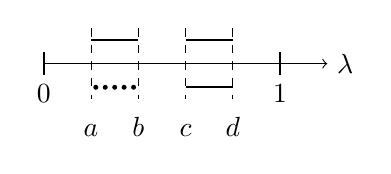
\begin{tikzpicture}[scale=3]

    % Axis
    \draw[->] (0,0) -- (1.2,0) node[right] {$\lambda$};

    % Tick marks and labels at 0 and 1
    \foreach \x/\label in {0/0, 1/1}
    {
        \draw[thick] (\x,0.05) -- (\x,-0.05);
        \node[below=4pt] at (\x,0) {$\label$};
    }

    % Two disjoint clusters
    \draw[thick] (0.2,0.1) -- (0.4,0.1);
    \draw[thick] (0.6,0.1) -- (0.8,0.1);
    % \node[above] at (0.3,0.1) {Cluster 1};
    % \node[above] at (0.7,0.1) {Cluster 2};
    % \node[left] at (0,0.1) {\small Two disjoint clusters};
    
    % Cluster with tail
    \draw[thick] (0.6,-0.1) -- (0.8,-0.1); % main cluster
    \foreach \x in {0.22,0.26,0.30,0.34,0.38} 
        \fill (\x,-0.1) circle (0.3pt); % tail eigenvalues
    % \node[below] at (0.7,-0.1) {Main cluster};
    % \node[below] at (0.3,-0.1) {Tail};
    % \node[left] at (0,-0.1) {\small Cluster with tail};
    
    % Mark points a, b, c, d
    \foreach \x/\label in {0.2/a, 0.4/b, 0.6/c, 0.8/d}
    {
        \draw[thin,dashed] (\x,0.15) -- (\x,-0.15);
        \node[above] at (\x,-0.35) {$\label$};
    }
    
\end{tikzpicture}
    \caption{Eigenspectrum of $A$ with two clusters and a tail of eigenvalues.}
    \label{fig:eigenvalue_clusters}
\end{figure}

The CG error \cref{eq:cg_error_bound} suggests we look for a polynomial $r_{m_2}$ of degree $m_2$ that satisfies the constraints of the minimization problem in order to find an iteration bound $m < m_2$. In other words, we do not solve the minimization problem directly, but we make a clever selection of the polynomial $r_{m_2}$ that satisfies the constraints. As a consequence, the actual minimizing polynomial might require a lower degree $m$ to satisfy the same relative error tolerance $\epsilon$. Therefore, the degree $m_2$ we find is at least as large as the actual number of iterations required to achieve the desired relative error tolerance $\epsilon$.

\citeauthor{cg_sharpened_convrate_Axelsson1976} suggests we use not one monolithic residual polynomial function, but a multiplication of two residual polynomial functions $\hat{r}^{(i)}_p(x)$ and $\hat{r}_{m_2-p}(x)$ for the two clusters. The superscript $^{(i)}$ corresponds to the two eigenspectra described above. The residual polynomial functions are defined using \cref{def:scaled_chebyshev_polynomial} and $\gamma = 0$ as follows
\begin{equation}
    \hat{r}^{(i)}_p (x)
    \begin{cases}
        \hat{C}_p&, \text{if } i = 1\\
        \overset{p}{\underset{i=1}{\prod}} (1 - x/\lambda_i)&, \text{if } i = 2, p = N_{\text{tail}}\\
    \end{cases}
    \label{eq:residual_polynomial_rm}
\end{equation}
and
\begin{equation}
    \hat{r}_{{m_2}-p} (x) = \frac{C_{m_2-p} \left(\frac{d + c - 2x}{d - c}\right)}{C_{m_2-p}\left(\frac{d + c}{d - c}\right)},
    \label{eq:residual_polynomial_rpm}
\end{equation}
Indeed, the product $r_{m_2} = \hat{r}_p \hat{r}_{m_2-p} \in \mathcal{P}_{m_2}$. Hence, we can use the residual polynomial functions to bound the error at the $m^{\text{th}}$ iterate. Now, we obtain the following intermediate bounds
\begin{subequations}
    \begin{align}
        \max_{\lambda \in [a,b]} |r_{m_2}(\lambda)| \leq \max_{\lambda \in [a,b]} |\hat{r}^{(i)}_p(\lambda)| \max_{\lambda \in [a,b]} |\hat{r}_{m_2-p}(\lambda)| &\leq \max_{\lambda \in [a,b]} |\hat{r}^{(i)}_p(\lambda)|, \ \text{and} \label{eq:residual_polynomial_bound_ab}\\
        \max_{\lambda \in [c,d]} |r_{m_2}(\lambda)| \leq \max_{\lambda \in [c,d]} |\hat{r}^{(i)}_p(\lambda)| \max_{\lambda \in [c,d]} |\hat{r}_{m_2-p}(\lambda)| &\leq \max_{\lambda \in [c,d]} |\hat{r}_{p}(\lambda)|/C_{m_2-p}\left(\frac{d+c}{d-c}\right) \label{eq:residual_polynomial_bound_cd}
    \end{align}
\end{subequations}
where the first result follows from the fact that $|\hat{r}_{m-p}(x)| < 1 \ \forall x \in [a,b]$ and the second result from 
\[
    \left|C_{m-p}\left(\frac{d+c -2x}{d-c}\right)\right| < 1 \ \forall x \in [c,d].
\]

Furthermore, using the equality \cref{eq:chebyshev_polynomial_approximation}, we have
\begin{equation}
    \frac{1}{C_{k}\left(\frac{z_1 + z_2}{z_1 - z_2}\right)} \leq 2 \left(\frac{\sqrt{z_2} - \sqrt{z_1}}{\sqrt{z_2} + \sqrt{z_1}}\right)^k, \text{ for } z_1 > z_2 > 0 \text{ and } k \in \mathbb{N}^+,
    \label{eq:chebyshev_polynomial_bound}
\end{equation}
and
\begin{equation}
    \max_{\lambda \in [a,b]} |\hat{r}^{(i)}_p(\lambda)| \leq
    \begin{cases}
        2\left(\frac{\sqrt{b}-\sqrt{a}}{\sqrt{b}+\sqrt{a}}\right)^p=\eta_1 &, \text{if } i = 1,\\
        \left(\frac{b}{a}-1\right)^p=\eta_2 &, \text{if } i = 2, p = N_{\text{tail}},
    \end{cases}
    \label{eq:residual_polynomial_bound_ab_i}
\end{equation}
Note that if $i=1$ we can determine $p$ by requiring that the maximum of the residual polynomial function $\hat{r}^{(i)}_p$ in $[a,b]$ is equal to $\epsilon$. This gives the following equation
\begin{equation}
    p \geq \left\lfloor\frac{1}{2}\sqrt{\frac{b}{a}}\ln{\frac{2}{\epsilon}} + 1\right\rfloor
    \label{eq:chebyshev_degree_p}
\end{equation}
Also note that for $i=2$ $\hat{r}^{(2)}_p(\lambda) = 0 < \epsilon$ for all eigenvalues $\lambda \in [a,b]$.

Next, $\hat{r}^{(i)}_p$ in $[c,d]$ is bounded by its maximum value within $[a,b]$ multiplied by the polynomial that is the fastest growing polynomial in $\mathcal{P}_{p}$ outside- and bounded below 1 within $[a,b]$. This polynomial is again the (transformed) Chebyshev polynomial $C_{p}\left(\frac{2x - b - a}{b - a}\right)$. Therefore,
\begin{equation*}
    \max_{\lambda \in [c,d]} |\hat{r}^{(i)}_p(\lambda)| \leq \eta_i C_{p}\left(\frac{2d - b - a}{b + a}\right),
\end{equation*}
with $\eta_i$ as defined in \cref{eq:residual_polynomial_bound_ab_i}.

At this point we have ensured that $\max_{\lambda \in [a,b]}|r_{m_2}|$ is bounded by $\epsilon$ using \cref{eq:residual_polynomial_bound_ab}. So it remains to bound $\max_{\lambda \in [c,d]}|r_{m_2}|$ in \cref{eq:residual_polynomial_bound_cd}. Using above results we can write 
\begin{equation*}
    \max_{\lambda \in [c,d]} |r_{m_2}(\lambda)| < \epsilon,
\end{equation*}
if we require that
\begin{equation}
    \eta_i C_{p}\left(\frac{2d - b - a}{b - a}\right) /C_{m_2-p}\left(\frac{d+c}{d-c}\right) < \epsilon.
    \label{eq:relative_error_bound_mp}
\end{equation}
Using that for $x_1, x_2, x_3 \in \mathbb{R}^+$ with $x_1 > x_3$ and $z = \frac{x_1 - x_2}{x_3}$
\begin{align*}
    C_p(z) & \leq \left(z + \sqrt{z^2 - 1}\right)^p \\
    & = \left( \frac{x_1 - x_2}{x_3} + \sqrt{ \left[\frac{x_1 - x_2}{x_3}\right]^2 -1}\right)^p \\
    & \leq \left( \frac{x_1}{x_3} + \sqrt{ \left[\frac{x_1}{x_3}\right]^2 - 1}\right)^p \\
    & \leq \left( \frac{2x_1}{x_3}\right)^p,
\end{align*}
and substituting $x_1 = 2d$, $x_2 = b + a$ and $x_3 = b - a$ we obtain the following inequality
\begin{equation}
    \eta_i \left(\frac{4d}{b-a} \right)^p /C_{m_2-p}\left(\frac{d+c}{d-c}\right) < \epsilon. 
    \label{eq:chebyshev_degree_p_bound}
\end{equation}
Moreover,
\begin{align*}
    \eta_i \left(\frac{4d}{b-a}\right)^p &= 
    \begin{cases}
        2\left(\frac{\sqrt{b} - \sqrt{a}}{\sqrt{b} + \sqrt{a}} \frac{4d}{b-a}\right)^p &, \text{if } i = 1\\
        \left(\frac{b - a}{a}\frac{4d}{b-a}\right)^p &, \text{if } i = 2,
    \end{cases}\\
    &=
    \begin{cases}
        2\left(\frac{4d}{b + 2\sqrt{ab} + a}\right)^p &, \text{if } i = 1\\
        \left(\frac{4d}{a}\right)^p &, \text{if } i = 2,
    \end{cases}\\
    &\leq 2
    \begin{cases}
        \left(\frac{4d}{b}\right)^p &, \text{if } i = 1\\
        \left(\frac{4d}{a}\right)^p &, \text{if } i = 2,
    \end{cases}
\end{align*}
We can therefore require that the bound in \cref{eq:chebyshev_degree_p_bound} is satisfied if we have
\[
    1/C_{m_2-p}\left(\frac{d+c}{d-c}\right) \leq \frac{\epsilon}{2\left( \frac{4d}{e_i}\right)^p},
\]
where 
\[
    e_i = \begin{cases}
        b &, \text{if } i = 1\\
        a &, \text{if } i = 2.\\
    \end{cases}
\]
Again using \cref{eq:chebyshev_polynomial_bound} and solving for the degree $m_2 - p$ we obtain
\[
    m_2 - p \geq \frac{1}{2}\sqrt{\frac{d}{c}}\left(\ln\left(\frac{2}{\epsilon}\right) + p \ln\left(\frac{4d}{e_i}\right)\right),
\]
which leads to the following bound for the number of iterations \cite[Equation 4.4]{cg_sharpened_convrate_Axelsson1976}
\begin{equation}
    m_2=\left\lfloor\frac{1}{2} \sqrt{\frac{d}{c}} \ln (2 / \epsilon)+\left(1+\frac{1}{2} \sqrt{\frac{d}{c}} \ln (4 d / e_i)\right) p\right\rfloor,
    \label{eq:cg_iteration_bound_2_clusters}
\end{equation}
where 
\[
    1 \leq p \leq \min\left(\left\lfloor\frac{1}{2}\sqrt{\frac{b}{a}}\ln{\frac{2}{\epsilon}} + 1 \right\rfloor, N_{\text{tail}}\right).
\]

\section{Performance ratio of the two-cluster bound}\label{sec:performance_ratio}
In this section we assume that we are dealing with an eigenspectrum of the form $\sigma_1(A)$, i.e. we are only treating case 1. For this case, we compare the new bound in \cref{eq:cg_iteration_bound_2_clusters} to the (approximated) classical bound in \cref{eq:cg_convergence_rate_bound_iterations_approx}. We will see that the new bound is not absolutely sharper than the classical one. However, we will derive an approximate, though accurate, criterion (see \cref{eq:threshold_inequality_explicit_expansion}) that allows us to discern under what conditions the new bound \textit{is} sharper.

To that end, we introduce a measure of performance as the ratio of the number of iterations predicted by the classical bound to that predicted by the sharpened bound
\begin{equation}
    P = \frac{m}{m_2}.
    \label{eq:performance_ratio}
\end{equation}
Consequently, the goal of this section is two-fold; determine the minimum value of $P$ and the conditions for which $P > 1$. We also introduce the left and right cluster condition numbers $\kappa_l = \frac{b}{a} > 1$ and $\kappa_r = \frac{d}{b} > 1$. Rewriting the bound from \cref{eq:cg_iteration_bound_2_clusters} in terms of the condition numbers gives
\[
    m_2(\kappa, \kappa_l, \kappa_r)=\left\lfloor\frac{\sqrt{\kappa_r}}{2} \ln (2 / \epsilon)+\left(1+\frac{\sqrt{\kappa_r}}{2} \ln \left(\frac{4\kappa}{\kappa_l}\right)\right) p\right\rfloor.
\]
Then, substituting $p$ gives
\begin{equation}
    m_2(\kappa, \kappa_l, \kappa_r)=\left\lfloor
        1 
        + \frac{\sqrt{\kappa_r}}{2}\ln\left(\frac{4\kappa}{\kappa_l}\right)
        + \frac{1}{2}\ln\left(\frac{2}{\epsilon}\right)\left(
            \sqrt{\kappa_l}
            + \sqrt{\kappa_r}
            + \frac{\sqrt{\kappa_l\kappa_r}}{2}\ln\left(\frac{4\kappa}{\kappa_l}\right)
        \right)
    \right\rfloor.
    \label{eq:cg_iteration_bound_2_clusters_condition_numbers}
\end{equation} 

\subsection{Uniform spectrum performance}\label{sec:cg_sharpened_convrate_uniform_performance}
In order to see that the new bound is not absolutely sharper than the classical one, we determine the minimum value of $P$. We know that the product of two lower order Chebyshev polynomials is not optimal for a uniform eigenspectrum, cf. the proof of Chebyshev optimality outlined in \cref{th:minmax_polynomial}. Therefore, we assume that the minimum value of $P$ is attained for the case of a uniform eigenspectrum, i.e. $a<b=c<d$, and we can set $\kappa=\kappa_l\kappa_r$, which yields
\begin{equation}
    m_2(\kappa=\kappa_l\kappa_r, \kappa_l, \kappa_r)=\left\lfloor
        1 
        + \frac{\sqrt{\kappa_r}}{2}\ln\left(4\kappa_r\right)
        + \underbrace{\frac{\sqrt{\kappa}}{2}\ln\left(\frac{2}{\epsilon}\right)}_{=m(\kappa)-1}\left(
            \underbrace{
                \frac{1}{\sqrt{\kappa_l}}
                + \frac{1}{\sqrt{\kappa_r}}
                + \frac{\ln\left(4\kappa_r\right)}{2}
            }_{:= q(\kappa_l, \kappa_r)}
        \right)
    \right\rfloor.
    \label{eq:cg_iteration_bound_2_clusters_uniform}
\end{equation}
We recognize the classical CG bound as the factor in front of the last term in \cref{eq:cg_iteration_bound_2_clusters_uniform}. Now, the performance ratio $P$ in \cref{eq:performance_ratio} satisfies
\begin{equation}
    P(\kappa=\kappa_l\kappa_r, \kappa_l, \kappa_r) = P_{\text{uniform}}(\kappa_l, \kappa_r) = \left(\frac{1 + \frac{1}{2}\sqrt{\kappa_r}\ln(4\kappa_r)}{m(\kappa_l\kappa_r)} + \frac{m(\kappa_l\kappa_r)-1}{m(\kappa_l\kappa_r)}q(\kappa_l, \kappa_r)\right)^{-1},
    \label{eq:performance_ratio_uniform}
\end{equation}
which can be expanded as
\[
    P_{\text{uniform}}(\kappa_l, \kappa_r) = \frac{m(\kappa_l\kappa_r)-1}{m(\kappa_l\kappa_r)}\left[q(\kappa_l, \kappa_r)^{-1} - \frac{1 + \frac{1}{2}\sqrt{\kappa_r}\ln(4\kappa_r)}{(m(\kappa_l\kappa_r)-1)q(\kappa_l, \kappa_r)^2} + \mathcal{O}\left(\frac{1}{(m(\kappa_l\kappa_r)-1)^2q(\kappa_l, \kappa_r)^3}\right)\right].
\]
Next, we require that $\kappa_r \gtrsim 5$, for which it holds that $\frac{1}{\sqrt{\kappa_l}} + \frac{1}{\sqrt{\kappa_r}} < \frac{\ln\left(4\kappa_r\right)}{2}, \ \forall \kappa_l \geq 1$. This requirement on $\kappa_r$ ensures that we can expand $q(\kappa_l, \kappa_r)^{-1}$ as follows
\[
    q(\kappa_l, \kappa_r)^{-1} = \frac{1}{\ln(4\kappa_r)} - \frac{1}{\ln(4\kappa_r)^2}\left(\frac{1}{\sqrt{\kappa_l}} + \frac{1}{\sqrt{\kappa_r}}\right) + \mathcal{O}\left(\frac{1}{(\ln(4\kappa_r))^3}\left(\frac{1}{\sqrt{\kappa_l}} + \frac{1}{\sqrt{\kappa_r}}\right)^2\right),
\]
which gives the performance for a uniform eigenspectrum as
\begin{align}
    P_{\text{uniform}}(\kappa_l, \kappa_r) &\approx \frac{1}{\ln(4\kappa_r)} \left(1 - \frac{1}{\sqrt{\kappa_l}\ln\left(\frac{2}{\epsilon}\right)}\right) \notag \\
    &\quad - \frac{1}{\ln(4\kappa_r)^2}\left(\frac{1}{\sqrt{\kappa_l}} + \frac{1}{\sqrt{\kappa_r}} + \frac{1}{\sqrt{\kappa_l\kappa_r}\ln\left(\frac{2}{\epsilon}\right)}\right) \notag \\
    &\quad + \mathcal{O}\left(\frac{1}{\ln(4\kappa_r)}\left[\frac{1}{\ln(4\kappa_r)^2} + \frac{1}{\kappa_l\kappa_r\ln\left(\frac{2}{\epsilon}\right)^2}\right]\right).
    \label{eq:performance_ratio_uniform_expansion}
\end{align}
The approximate equality in \cref{eq:performance_ratio_uniform_expansion} stems from the fact that
\[
    \frac{m(\kappa_l\kappa_r)-1}{m(\kappa_l\kappa_r)} \underset{\kappa_l\kappa_r \geq 5}{\approx} 1.
\]

Equation \ref{eq:performance_ratio_uniform_expansion} shows that the uniform (minimum) performance $P_{\text{uniform}}(\kappa_l, \kappa_r)$ tends in its leading order term to $1/\ln(4\kappa_r)$ as $\kappa_l \to \infty$. That is, let $P^{(i)}_{\text{uniform}}$ denote the $i$-th order expansion of \cref{eq:performance_ratio_uniform_expansion}, then
\[
    P_{\text{uniform}}(\kappa_l, \kappa_r) \lesssim \frac{1}{\ln(4\kappa_r)} = P^{(0)}_{\text{uniform}}(\kappa_r).
\]
Only for small $\kappa_l = \frac{\kappa}{\kappa_r}$ does the first order term become significant. Additionally, \cref{eq:performance_ratio_uniform_expansion} shows that for increasing $\kappa_r$ we expect a decreasing minimum performance. We also find that the new bound $m_2(\kappa,\kappa_l,\kappa_r)$ is not absolutely sharper than the classical bound $m(\kappa)$. In fact, based on the terms in the expansion of \cref{eq:performance_ratio_uniform_expansion} we can say that
\begin{equation}
    P^{(1)}_{\text{uniform}}(\kappa_l, \kappa_r) \lesssim P_{\text{uniform}}(\kappa_l, \kappa_r) \lesssim P^{(0)}_{\text{uniform}}(\kappa_r),
    \label{eq:performance_ratio_no_improvement_bounds}
\end{equation}

\subsection{Performance threshold}\label{sec:performance_threshold}
Now that we have established that the new bound is not absolutely sharper than the classical one, we can determine the conditions under which the new bound is sharper. We know that for $\kappa=\kappa_r\kappa_l$ the performance ratio $P$ is given by \cref{eq:performance_ratio_uniform}. We now solve the inverse problem, i.e. for what $\kappa$ is $P \geq 1$? This gives the following inequality
\[
    \frac{m}{m_2} \geq 1 \Rightarrow m(\kappa) \geq m_2(\kappa, \kappa_l, \kappa_r),
\]
which can be rewritten as
\begin{equation}
    \sqrt{\frac{\kappa}{\kappa_l\kappa_r}} \geq \frac{1}{2}\ln\left(\frac{4\kappa}{\kappa_l}\right) + \frac{1}{\sqrt{\kappa_r}} + \frac{1}{\sqrt{\kappa_l}}\left(1 + \log_{\frac{2}{\epsilon}}\left(\frac{4\kappa}{\kappa_l}\right)\right).
    \label{eq:threshold_inequality}
\end{equation}
At this point we neglect the last term in \cref{eq:threshold_inequality}. Doing so relaxes the constraint on the performance ratio as
\begin{equation}
    P \geq 1 - \mathcal{O}\left(\sqrt{\frac{\kappa_r}{\kappa_l}}\log_{\frac{2}{\epsilon}}\left(\frac{4\kappa}{\kappa_l}\right)\right) = P_{\text{threshold}},
    \label{eq:approximate_performance_ratio_threshold}
\end{equation}
which is a good approximation as long as $\kappa_l \geq \kappa \gg 1$. Next to simplifying \cref{eq:threshold_inequality}, this reduces the number of variables. Indeed, by introducing a new parameter for the \textit{spectral width} $s = \frac{\kappa}{\kappa_l}$, dropping the last term in \cref{eq:threshold_inequality} and setting $c_r = \frac{2}{\sqrt{\kappa_r}}$ we can write
\begin{equation}
    c_r\sqrt{s} \geq \ln\left(4s\right) + c_r.
    \label{eq:threshold_inequality_s}
\end{equation}
We use the Lambert $\mathrm{W}$ function to solve the equality in \cref{eq:threshold_inequality_s} for $s$. In order to do so, we transform the equality into the form $x = y \mathrm{e}^y$ with $y = -\frac{c_r\sqrt{s}}{2}$ and $x = -\frac{c_r}{4\exp\left(\frac{c_r}{2}\right)}$. Then, we can write
\begin{align*}
    -\frac{c_r\sqrt{s}}{2} = y = W_{-1}(x) = W_{-1}\left(-\frac{c_r}{4\exp\left(\frac{c_r}{2}\right)}\right), \quad x \in \left(-\frac{1}{\mathrm{e}}, 0 \right],
\end{align*}
where $W_{-1}$ is the first negative branch of the Lambert $\mathrm{W}$ function. The condition on $x$ ensures that $W_{-1}$ evaluates to a real number. Note that $\kappa_r\geq1 \implies c_r \leq 1$. So the condition on $x$ is indeed satisfied. Finally, after substituting $c_r = \frac{2}{\sqrt{\kappa_r}}$ we obtain an explicit expression for the spectral width $s$ in terms of the right cluster condition number $\kappa_r$
\[
    s(\kappa, \kappa_l) \geq \kappa_r W_{-1}\left(-\frac{1}{2\sqrt{\kappa_r}\exp\left(\frac{1}{\sqrt{\kappa_r}}\right)}\right)^2,
\]
or, in terms of the original condition numbers
\begin{equation}
    \kappa \geq 4\kappa_l\kappa_r W_{-1}\left(-\frac{1}{2\sqrt{\kappa_r}\exp\left(\frac{1}{\sqrt{\kappa_r}}\right)}\right)^2 = T_{\kappa}(\kappa_l, \kappa_r).
    \label{eq:threshold_inequality_explicit}    
\end{equation}
The evaluation of the Lambert $\mathrm{W}$ function is not a trivial task and often requires numerical methods for accurate computation \cite{evaluation_of_the_lambert_w_function_Corless1996}. Luckily, there exists an expansion of $\mathrm{W}_{-1}(x)$ for $x\rightarrow0^-$ \cite[Equation 4.19]{evaluation_of_the_lambert_w_function_Corless1996}. Let $x$ be as above and set $L = \ln(-x)$ and $l = \ln(-L)$, then
\begin{equation}
    \kappa \geq 4\kappa_l\kappa_r \left(L - l + \frac{l}{L}\right)^2 + \mathcal{O}\left(\frac{\kappa_l\kappa_rl^4}{L^4}\right) := T^{(0)}_{\kappa}(\kappa_l, \kappa_r) + \mathcal{O}\left(\frac{\kappa_l\kappa_rl^4}{L^4}\right).
    \label{eq:threshold_inequality_explicit_expansion}    
\end{equation}

Combining the results of this section with those of \cref{sec:cg_sharpened_convrate_uniform_performance} we can now say that as long as $\kappa_l\kappa_r \leq \kappa \leq T_{\kappa}(\kappa_l, \kappa_r)$, the performance ratio satisfies
\begin{equation}
    P_{\text{uniform}}(\kappa_l, \kappa_r) \leq P(\kappa, \kappa_l, \kappa_r) \leq P_{\text{threshold}} \lesssim 1,
    \label{eq:performance_bounds}
\end{equation}
and, conversely, if $\kappa > T_{\kappa}(\kappa_l, \kappa_r)$, then 
\[
    P(\kappa, \kappa_l, \kappa_r) > P_{\text{threshold}}
\]

\subsection{Performance plot}
Figure \ref{fig:two_cluster_bound_performance} visualizes all the findings regarding the performance of the two-cluster bound $m_2$. 
\begin{figure}[H]
    \centering
    \includegraphics[width=\textwidth]{performance_vs_condition_number.pdf}
    \caption{Performance ratio of the classical bound $m$ from \cref{eq:cg_convergence_rate_bound_iterations_approx} and the new two-cluster bound $m_2$ from \cref{eq:cg_iteration_bound_2_clusters} as a function of the global condition number $\kappa$ for right cluster condition number $\kappa_r = 5$ (\textbf{left}) and $\kappa_r = 10^3$ (\textbf{right}). All plots contain graphs for spectra with $\kappa_l = 1, 10, 10^2, 10^3, 10^4$. The plots also contain a red, shaded region for which $P_{\text{uniform}} < P < 1$, a diagonally hashed region resembling the performance bounds from \cref{eq:performance_bounds}, a red, dashed line resembling the first order expansion of the uniform performance ratio, $P^{(1)}_{\text{uniform}}$ from \cref{eq:performance_ratio_uniform_expansion}, and both the exact and approximate $\kappa$-threshold values for each $\kappa_l$ graph from \cref{eq:threshold_inequality_explicit,eq:threshold_inequality_explicit_expansion}, respectively.}
    \label{fig:two_cluster_bound_performance}
\end{figure}
We can notice that the performance graphs for various left cluster widths $\kappa_l$ grow with the square root of the global condition number, i.e. $P \approx \mathcal{O}(\sqrt{\kappa})$, as the slope of these lines is approximately $1/2$. This is to be expected from \cref{eq:cg_iteration_bound_2_clusters_condition_numbers}, since for constant $\kappa_l,\kappa_r$, and $\kappa > T_h(\kappa_l, \kappa_r) \gg 1$ we have that $P = \mathcal{O}\left(\frac{\sqrt{\kappa}}{\ln(4\kappa)}\right)$. The slope of the term $\frac{\sqrt{\kappa}}{\ln(4\kappa)}$ in a log-log plot satisfies
\[
    \frac{d\ln(P)}{d\ln(\kappa)} =\kappa\frac{d\ln(P)}{d\kappa} \sim \kappa\frac{d}{d\ln(\kappa)} \left[\ln(\sqrt{\kappa}) - \ln(\ln(4\kappa))\right] = \frac{1}{2} - \frac{1}{\ln(4\kappa)} \underset{\kappa\to\infty}{\longrightarrow} \frac{1}{2}.
\]
Next to this we can see that the first order expansion of the uniform performance ratio $P^{(1)}_{\text{uniform}}$ agrees well with the minimum performance bound as long as $\kappa = \kappa_l\kappa_r \gg 1$, which is in agreement with the error terms in \cref{eq:performance_ratio_uniform_expansion} and the minimum performance bound from \cref{eq:performance_bounds}. Finally, we see that both $T_{\kappa}(\kappa_l, \kappa_r)$ and its zeroth order expansion $T^{(0)}_{\kappa}(\kappa_l, \kappa_r)$ from \cref{eq:threshold_inequality_explicit,eq:threshold_inequality_explicit_expansion} are accurate approximations of the actual $\kappa$-threshold value at which $P=1$, and even more so for larger values of $\kappa,\kappa_r$. We do see a deviation of both $T_{\kappa}(\kappa_l, \kappa_r)$ and $T^{(0)}_{\kappa}(\kappa_l, \kappa_r)$ for $\kappa_l\leq\kappa_r$. Again, this is in agreement with the error terms in \cref{eq:approximate_performance_ratio_threshold}.

\section{Performance of the tail-cluster bound}\label{sec:tail_cluster_bound_performance}
The two-cluster bound from \cref{eq:cg_iteration_bound_2_clusters} is also derived for the case of a right cluster with a tail of eigenvalues $\sigma_2$, i.e. the case where the left cluster is a tail cluster. In this case, we can also derive a minimum performance ratio $P^{\text{tail}}_{\text{uniform}}$. We again consider a uniform spectrum, i.e. $a<b=c<d$, and we can set $\kappa=\kappa_l\kappa_r$. The tail-cluster bound is given by \cref{eq:cg_iteration_bound_2_clusters} with $p = N_{\text{tail}} \leq \left\lfloor\frac{\sqrt{\kappa_l}}{2}\ln{\frac{2}{\epsilon}} + 1 \right\rfloor $. This gives
\[
    m_2(\kappa=\kappa_l\kappa_r, p, \kappa_r) = \left\lfloor
        \frac{\sqrt{\kappa_r}}{2}\ln\left(\frac{2}{\epsilon}\right) 
        + p \left(
            1 + \frac{\sqrt{\kappa_r}}{2}\ln\left(\frac{4\kappa}{\kappa_l}\right)
        \right)
    \right\rfloor.
\]
The performance ratio $P^{\text{tail}}_{\text{uniform}}$ is given by
\begin{equation}
    P^{\text{tail}}_{\text{uniform}}(\kappa_l, \kappa_r) = \frac{\sqrt{\kappa_l}\ln\left(\frac{2}{\epsilon}\right)}{p\ln(4\kappa_r)} - \mathcal{O}\left(\frac{\sqrt{\kappa_l}\ln\left(\frac{2}{\epsilon}\right)}{p^2\ln(4\kappa_r)^2}\right), \quad \text{for } \kappa_l \geq \kappa_r < \frac{1}{2\epsilon}.
    \label{eq:performance_ratio_tail_uniform}
\end{equation}
Equation \ref{eq:performance_ratio_tail_uniform} shows that
\[
    P^{\text{tail}}_{\text{uniform}}(\kappa_l, \kappa_r) \longrightarrow \frac{1}{\ln(4\kappa_r)} = P^{(0)}_{\text{uniform}}(\kappa_r) \quad \text{as } p \to \left\lfloor\frac{\sqrt{\kappa_l}}{2}\ln{\frac{2}{\epsilon}} + 1 \right\rfloor,
\]
that is, the minimum performance of the tail-cluster bound reduces to the two-cluster bound as $p$ approaches its maximum value. Another crucial aspect about $P^{\text{tail}}_{\text{uniform}}(\kappa_l, \kappa_r)$ is found when we require the leading order term to be larger than $1$, giving us the following inequality
\begin{equation}
    p < \sqrt{\kappa_l}\log_{4\kappa_r}\left(\frac{2}{\epsilon}\right).
    \label{eq:tail_cluster_bound_sparsity_condition}
\end{equation}
Equation \ref{eq:tail_cluster_bound_sparsity_condition} can be interpreted as a \textit{sparsity condition} on the tail cluster, i.e. the tail cluster must be sparse enough to ensure that the performance ratio is larger than $1$.

\section{Generalization to multiple clusters}\label{sec:multiple_clusters}
The technique outlined in \cref{sec:cg_sharpened_convrate} starts at the left most cluster $[a,b]$, finds the Chebyshev degree $p_1=p$ satisfying \cref{eq:chebyshev_degree_p}, moves to the neighboring cluster $[c,d]$ and finds the Chebyshev degree $p_2 = m_2 - p$ satisfying \cref{eq:relative_error_bound_mp}. Rewriting \cref{eq:relative_error_bound_mp} gives the following equation for $p_2$:
\begin{equation}
    \frac{1}{C_{p_2}\left(\frac{d+c}{d-c}\right)} \leq \frac{\epsilon}{{C}^{(1)}_{p_1}(d)} = \epsilon_2,
    \label{eq:chebyshev_degree_p_prime}
\end{equation}
where
\[
    C^{(1)}_{p_1}(x) = C_{p_1}\left(\frac{b + a - 2x}{b - a}\right) /C_{p_1}\left(\frac{b+a}{b-a}\right),
\]
is the Chebyshev polynomial corresponding to the first cluster.

Suppose there is a third cluster to the right of $[c,d]$, i.e. $[e,f]$. We can repeat the process and find the Chebyshev degree $p_3$ satisfying a similar equation as \cref{eq:chebyshev_degree_p_prime} for the third cluster. 
\[
    \frac{1}{C_{p_3}\left(\frac{f+e}{f-e}\right)} \leq \frac{\epsilon}{C^{(1)}_{p_1}(f)C^{(2)}_{p_2}(f)} = \epsilon_3,
\]
This leads to the general equation for the Chebyshev degree $p_i$ of the $i^{\text{th}}$ cluster $[a_i, b_i]$
\begin{equation}
    \frac{1}{C_{p_i}\left(\frac{b_i + a_i}{b_i - a_i}\right)} \leq \frac{\epsilon}{\prod_{j=1}^{i-1} C^{(j)}_{p_j}(b_i)} = \epsilon_i.
    \label{eq:chebyshev_degree_p_i}
\end{equation}

The Chebyshev polynomials $\tilde{C}_p$ grow rapidly outside the interval $[-1,1]$ \cite[Section 4]{cg_sharpened_convrate_Axelsson1976}. Therefore, it can be cumbersome for a computer to evaluate the product of the $C^{(j)}_{p_j}(b_i)$ terms in the denominator of \cref{eq:chebyshev_degree_p_i}, as it might result in floating-point number overflow. Instead, we first apply \cref{eq:chebyshev_polynomial_bound} and introduce the cluster condition numbers $\kappa_i = \frac{b_i}{a_i}$, where $i$ is the index of the cluster. We can then rewrite \cref{eq:chebyshev_degree_p_i} using \cref{eq:chebyshev_polynomial_approximation} as follows
\begin{equation*}
    p_i  =  \left\lceil\ln{\frac{\epsilon_i}{2}} / \ln{\frac{\sqrt{\kappa_i} - 1}{\sqrt{\kappa_i} + 1}}\right\rceil, \\
\end{equation*}
and
\begin{align*}
    \ln{\frac{\epsilon_i}{2}} & = \ln{\frac{\epsilon}{2}} - \sum_{j=1}^{i-1} \ln{C^{(j)}_{p_j}(b_i)}. \\
\end{align*}
Let $z^{(i,j)}_1 = \frac{b_j + a_j - 2b_i}{b_j - a_j}$ and $z^{(j)}_2 = \frac{b_j + a_j}{b_j - a_j}$ then
\begin{equation*}
    \ln{C^{(j)}_{p_j}(b_i)} = \ln{C_{p_j}(z^{(i,j)}_1)} - \ln{C_{p_j}(z^{(j)}_2)}.
\end{equation*}
We have, using the approximations in \cref{eq:chebyshev_polynomial_approximation}
\begin{equation}
    \ln{C_{p_j}(z^{(i,j)}_1)} \approx p_j \ln{\left|z^{(i,j)}_1 - \sqrt{\left(z^{(i,j)}_1\right)^2 - 1}\right|} - \ln{2},
    \label{eq:chebyshev_polynomial_bound_z1}
\end{equation}
and
\begin{equation}
    \ln{C_{p_j}(z^{(j)}_2)} \approx p_j \ln{\left[z^{(j)}_2 + \sqrt{\left(z^{(j)}_2\right)^2 - 1}\right]} - \ln{2},
    \label{eq:chebyshev_polynomial_bound_z2}
\end{equation}
both of which become more accurate approximations as $z,m\rightarrow\infty$. Introducing 
\begin{align*}
    \zeta^{(i,j)}_1 &= z^{(i,j)}_1 - \sqrt{\left(z^{(i,j)}_1\right)^2 - 1}, \\
    \zeta^{(j)}_2 &= z^{(j)}_2 + \sqrt{\left(z^{(j)}_2\right)^2 - 1}, \text{ and}\\
    f_i &= \frac{\sqrt{\kappa_i} - 1}{\sqrt{\kappa_i} + 1},
\end{align*}
with $\kappa_i$ the $i^{\text{th}}$ cluster condition number, and substituting the inequalities \ref{eq:chebyshev_polynomial_bound_z1} and \ref{eq:chebyshev_polynomial_bound_z2} back into the bound for $p_i$ gives
\begin{align*}
    p_i &\leq \left\lceil\frac{\ln{\frac{\epsilon}{2}} - \sum_{j=1}^{i-1} p_j\left(\ln{\zeta^{(i,j)}_1} - \ln{\zeta^{(j)}_2} \right)}{\ln{f_i}}\right\rceil \\
    &= \left\lceil\log_{f_i}{\frac{\epsilon}{2}} - \sum_{j=1}^{i-1} p_j\left(\log_{f_i}{\zeta^{(i,j)}_1} - \log_{f_i}{\zeta^{(j)}_2} \right)\right\rceil\\
    &= \left\lceil\log_{f_i}{\frac{\epsilon}{2}} - \sum_{j=1}^{i-1} p_j\log_{f_i}{\frac{\zeta^{(i,j)}_1}{\zeta^{(j)}_2}} \right\rceil
\end{align*}
Note that in general $f_i < 1$ and $\zeta^{(i,j)}_1 > \zeta^{(j)}_2$. Therefore, term $\log_{f_i}{\left(\frac{\zeta^{(i,j)}_1}{\zeta^{(j)}_2}\right)} < 0$. So we multiply this term by $-1$ and obtain
\begin{equation}
    p_i \leq \left\lceil\log_{f_i}{\frac{\epsilon}{2}} + \sum_{j=1}^{i-1} p_j\log_{f_i}{\frac{\zeta^{(j)}_2}{\zeta^{(i,j)}_1}} \right\rceil
    \label{eq:chebyshev_degree_p_i_explicit}
\end{equation}
Evidently, adding more clusters to the left of the interval $[a_i,b_i]$ increases the degree $p_i$ of the Chebyshev polynomial. Next to this, \cref{eq:chebyshev_degree_p_i_explicit} reduces to the classical CG iteration bound \cref{eq:cg_convergence_rate_bound_iterations} for a single cluster when $i = N_{\text{clusters}} = 1$.

Equation \ref{eq:chebyshev_degree_p_i_explicit} gives us a way to calculate the Chebyshev degree $p_i$ of the $i^{\text{th}}$ cluster $[a_i,b_i]$ in terms of the Chebyshev degrees of the previous clusters. To obtain a bound on the number of iterations for the CG method we sum the Chebyshev degrees of all the clusters
\begin{equation}
    m_{N_{\text{clusters}}} = \sum_{i=1}^{N_{\text{clusters}}} p_i
    \label{eq:cg_iteration_bound_multiple_clusters}
\end{equation}

We summarize the techniques outlined in this section in \cref{alg:multi_cluster_bound}. The algorithm takes a set of clusters and a relative error tolerance $\epsilon$ as input and returns the multi-cluster CG bound $m_{N_{\text{clusters}}}$. The algorithm iterates over all clusters, calculating the Chebyshev degree $p_i$ for each cluster based on the previous clusters' degrees and the relative error tolerance. Finally, it sums up all the degrees to obtain the multi-cluster CG bound.
\begin{algorithm}[H]
    \caption{$\operatorname{MultiClusterCGIterationBound}(\text{clusters}, \epsilon)$}
    \begin{algorithmic}[1]
        \State \textbf{Input:} Sorted set $\text{clusters} = \langle[a_1, b_1], [a_2, b_2], \ldots, [a_{N_{\text{clusters}}}, b_{N_{\text{clusters}}}]\rangle$ and relative error tolerance $\epsilon$
        \State \textbf{Output:} Multi-cluster CG bound $m_{N_{\text{clusters}}}$
        \State Initialize $P \gets \emptyset$
        \For{$[a_i, b_i] \in \text{clusters}$} 
            \State $\epsilon_i \gets \ln(\epsilon)$
            \For{$[a_j, b_j] \in \text{clusters}_{<i}$} \Comment{$\text{clusters}_{<i}$ = all clusters to the left of $[a_i, b_i]$}
                \State $z_1 \gets \frac{b_j + a_j - 2b_i}{b_j - a_j}$
                \State $z_2 \gets \frac{b_j + a_j}{b_j - a_j}$
                \State $p_j \gets P[j]$
                \State $\epsilon_i \gets \epsilon_i - p_j \left(\ln(z_1^2 -1) - \ln\left(z_2 + \sqrt{z_2^2 -1}\right)\right)$
            \EndFor
            \State $f_i \gets \frac{\sqrt{\kappa_i} - 1}{\sqrt{\kappa_i} + 1}$, where $\kappa_i = \frac{b_i}{a_i}$
            \State $p_i \gets \left\lceil\log_{f_i}\left(\frac{\epsilon_i}{2}\right)\right\rceil$
            \State $P \gets P \cup \langle p_i \rangle$
        \EndFor
        \State $m_{N_{\text{clusters}}} \gets \sum_{i=1}^{N_{\text{clusters}}} P[i]$
        \State \Return $m_{N_{\text{clusters}}}$
    \end{algorithmic}
    \label{alg:multi_cluster_bound}
\end{algorithm}

\section{Algorithm for sharpened CG bound}\label{sec:cg_sharpened_convrate_multiple_clusters_algorithm}
In this section we combine the findings of \cref{sec:performance_ratio,sec:multiple_clusters} to derive a flexible algorithm for determining a sharpened CG bound. The idea is to use a simple algorithm to split the eigenspectrum into two clusters. Then, we calculate the left and right cluster condition numbers $\kappa_l$ and $\kappa_r$ and check if the approximate threshold condition in \cref{eq:threshold_inequality_explicit_expansion} is satisfied. In fact, the algorithm will recursively apply the previous two steps, stopping only when the threshold condition is not satisfied. The result is a list of indices at which to split the eigenspectrum, yielding an ordered set of clusters $\langle[a_i, b_i]\rangle_{i=1}^{N_{\text{clusters}}}$, where $N_{\text{clusters}}$ is the number of clusters. Finally, the algorithm computes the Chebyshev degrees $p_i$ for each cluster using \cref{eq:chebyshev_degree_p_i_explicit} and sums these up to obtain the sharpened CG bound $m_{N_{\text{clusters}}}$.

Given an eigenspectrum $\sigma = \{\lambda_1, \lambda_2, \ldots, \lambda_n\}$ with $0 < \lambda_1 \leq \lambda_2 \leq \cdots \leq \lambda_n$, we need to determine a split point. We choose to split the eigenspectrum at the \textit{largest logarithmic gap} between consecutive eigenvalues.
\begin{algorithm}[H]
    \caption{$\operatorname{SplitEigenspectrum}(\sigma)$}
    \begin{algorithmic}[1]
        \State \textbf{Input:} Sorted eigenvalues $\sigma = \langle\lambda_1, \lambda_2, \ldots, \lambda_n\rangle$ with $\lambda_i > 0$
        \State \textbf{Output:} Split index $k^*$ such that clusters are $\langle\lambda_1, \ldots, \lambda_{k^*}\rangle$ and $\langle\lambda_{k^*+1}, \ldots, \lambda_n\rangle$
        \State Initialize $\text{max\_gap} \gets 0$, $k^* \gets 1$
        \For{$i = 1$ to $n-1$}
            \State Compute logarithmic gap: $g_i \gets \ln(\lambda_{i+1}) - \ln(\lambda_i) = \ln\left(\frac{\lambda_{i+1}}{\lambda_i}\right)$
            \If{$g_i > \text{max\_gap}$}
                \State $\text{max\_gap} \gets g_i$
                \State $k^* \gets i$
            \EndIf
        \EndFor
        \State \Return $k^*$
    \end{algorithmic}
    \label{alg:split_eigenspectrum}
\end{algorithm}
The logarithmic criterion in \cref{alg:split_eigenspectrum} is particularly suitable for eigenspectra because it accounts for the relative scaling of eigenvalues, which is important when dealing with condition numbers of vastly different magnitudes.

Recursive application of \cref{alg:split_eigenspectrum} with stopping criterion based on the threshold condition in \cref{eq:threshold_inequality_explicit_expansion} leads to \cref{alg:partition_eigenspectrum}.
\begin{algorithm}[H]
    \caption{$\operatorname{PartitionEigenspectrum}(\sigma)$}
    \begin{algorithmic}[1]
        \State \textbf{Input:} Sorted eigenvalues $\sigma = \langle\lambda_1, \lambda_2, \ldots, \lambda_n\rangle$
        \State \textbf{Output:} Sorted partition indices $K^* = \langle k^*_1, k^*_2, \ldots, k^*_{N_{\text{clusters}}-1}, n\rangle$
        \State $\kappa \gets \frac{\lambda_n}{\lambda_1}$
        \State $k^* \gets \operatorname{SplitEigenspectrum}(\sigma)$
        \State $\kappa_l \gets \frac{\lambda_{k^*}}{\lambda_1}$
        \State $\kappa_r \gets \frac{\lambda_n}{\lambda_{k^*+1}}$
        \If{$\kappa > T^{(0)}(\kappa_l,\kappa_r)$}
            \State \Return $\operatorname{PartitionEigenspectrum}(\sigma_{\leq k^*}) \cup k^* + 1 + \operatorname{PartitionEigenspectrum}(\sigma_{>k^*})$
        \Else
            \State \Return $\langle n \rangle$ \Comment{No further partitioning needed, return last index}
        \EndIf
    \end{algorithmic}
    \label{alg:partition_eigenspectrum}
\end{algorithm}
Note that \cref{alg:partition_eigenspectrum} returns at a minimum a set containing only the last index $K^*= \langle n \rangle$, if the threshold condition is not satisfied for any split. Additionally, the value $k^* + 1$ is added (element-wise) to the result of the right-hand recursion in line 8 of \cref{alg:partition_eigenspectrum}. This is to ensure that the resulting set of indices $K^*$ contains the correct, global indices of the eigenspectrum, as the right-hand recursion only returns indices relative to the right-hand side of the split.

Finally, we can combine the partitioning from \cref{alg:partition_eigenspectrum} with the Chebyshev degree calculation from \cref{alg:multi_cluster_bound} to obtain the sharpened CG bound \cref{alg:sharpened_cg_bound}.
\begin{algorithm}[H]
    \caption{$\operatorname{SharpenedCGIterationBound}(\sigma, \epsilon)$}
    \begin{algorithmic}[1]
        \State \textbf{Input:} Sorted eigenvalues $\sigma = \{\lambda_1, \lambda_2, \ldots, \lambda_n\}$, target relative error $\epsilon$
        \State \textbf{Output:} Sharpened CG iteration bound $m_{N_{\text{clusters}}}$
        \State Initialize $\text{clusters} \gets \emptyset$, $k_a \gets 1$
        \State $K^* \gets \operatorname{PartitionEigenspectrum}(\sigma)$
        \For{$k_b \in K^*$}
            \State $\text{clusters} \gets \text{clusters} \cup \langle[\sigma[k_a], \sigma[k_b]]\rangle$
            \State $k_a \gets k_b + 1$
        \EndFor
        \State \Return $\operatorname{MultiClusterCGIterationBound}(\text{clusters}, \epsilon)$
    \end{algorithmic}
    \label{alg:sharpened_cg_bound}
\end{algorithm}
Algorithm \ref{alg:sharpened_cg_bound} first partitions the eigenspectrum into clusters using \cref{alg:partition_eigenspectrum}. Then, it constructs a list of clusters and finally computes the sharpened CG bound using \cref{alg:multi_cluster_bound}. In the case that the eigenspectrum is never partitioned, i.e. the threshold condition is never satisfied, the algorithm returns the classical CG bound $m(\kappa)$ from \cref{eq:cg_convergence_rate_bound_iterations}.